\documentclass[runningheads]{llncs}

\renewcommand{\labelenumii}{\theenumii}
\renewcommand{\theenumii}{\theenumi.\arabic{enumii}.}

\usepackage{graphicx}
\usepackage{hyperref} %might be better to uncomment this
\usepackage{subfig}
\usepackage{listings}

% Used for displaying a sample figure. If possible, figure files should
% be included in EPS format.
%
% If you use the hyperref package, please uncomment the following line
% to display URLs in blue roman font according to Springer's eBook style:
\renewcommand\UrlFont{\color{blue}\rmfamily}

\begin{document}
%
%\title{Contribution Title\thanks{Supported by organization x.}}
\title{EARIN\\Laboratory report\\EXERCISE 6: Reinforcement learning}
%
%\titlerunning{very very very }
% If the paper title is too long for the running head, you can set
% an abbreviated paper title here
\author{Bartłomiej Mastej \& Paweł Borsukiewicz}
%
\institute{Warsaw University of Technology, Warsaw, Poland}

%
\maketitle              % typeset the header of the contribution
%
%
%
%
\begin{centering}
  {\huge
    Final results can be observed here:\\
    \href{https://www.youtube.com/watch?v=ed-zkrwlk8g}{Game won video}\\
    \href{https://www.youtube.com/watch?v=Ee54wHfOUyA}{Evaluation video}\\
  }
  (click on reference link to open the video)\\
\end{centering}
\section{Introduction}
The aim of the experiment was to train reinforcement learning models based on CarRacing-v0 environment and subsequently assess and compare their results. There was prepered the environment using the openAI gym for the 'CarRacing-v0' problem. Further, there was created the Proximal Policy Optimization model which was further tuned with the usage of the Grid Search algorithm. Finally, the results are assessed and concluded.

\section{Implementation}
First of all, there was prepared environment using the openAI gym environment. It was decided to use 'CarRacing-v0' gym instead of 'CarRacing-v1' due to high availability of libraries supporting reinforcement learning.
\subsection{Prerequisites}
At the very beginning, there was a need to configure the environment to work properly with the $gym$ module as well as with the $stable\textunderscore baselines3$. Furthermore, in order to make all modules work, the proper version of each of them had to be installed. The final configuration of the environment is presented on the Fig.~\ref{fig:libraries}.
\begin{figure}
  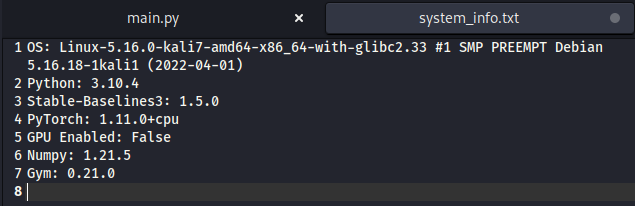
\includegraphics[width=\textwidth]{Screenshots/libraries.png}
  \caption{Configured environment parameters \& libraries}
  \label{fig:libraries}
\end{figure}

\subsection{Model \& learning procedure}
It was decided to use the PPO - Proximal Policy Optimization model from the $stable\textunderscore baselines3$ python module due to the ease of implementation and tuning. Furthermore, this module is implemented with the usage of the $TensorFlow$ module, hence the learning can be done with the GPU computational support. The implementation of the model creation with the parameters tuning is presented on the Listing.~\ref{lst:model}. Further, there was used the $learn$ method of the module which take the timestep as the parameter. The duration of the model learning is being saved as shown on the Listing.~\ref{lst:model}.

During the reinforcement learning process the network is being trained with the reward, hence in this exercise the positive reward is being given to a car while it drives through the tiles on the track, and the negative reward is being given if the car drives through the tiles off the track. The detailed reward policy is presented on the Fig.~\ref{fig:reward} It was implemented with the function $evaluate\textunderscore policy$, also from the $stable\textunderscore baselines3$ module, which returns the mean reward and the standard deviation. It is presented in the Listing.~\ref{lst:model}. Finally, as described in the subsection 3 the best model is being saved to a zip file.


\begin{lstlisting}[caption={Model creation}, language=Python, label={lst:model}]
  #Prepare model
  model = PPO(params['policy'], \
              env,\
              verbose=0, \
              learning_rate=params['l_rate'], \
              tensorboard_log=log_path, seed=2137, \
              n_steps=params['n_steps'], \
              n_epochs=params['n_epochs'])

  #Perform learning procedure
  print("LEARNING", iter, "/", len(grid))
  start = timeit.default_timer()
  model.learn(total_timesteps=params['timesteps'])
  stop = timeit.default_timer()
  l_time = "{0:0.3f}".format(stop - start)

  #Evaluate learning outcomes
  print("EVALUATING", iter, "/", len(grid))
  #Returns (Mean reward, Standard deviation)
  #Change render to true to see results
  mean, std = evaluate_policy(model, env,\
                              n_eval_episodes=3, \
                              render=False)
  print("Result:", mean)
\end{lstlisting}

\begin{figure}
  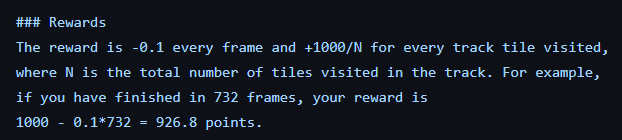
\includegraphics[width=\textwidth]{Screenshots/rewards.png}
  \caption{Reward policy}
  \label{fig:reward}
\end{figure}
\subsection{Grid Search parameters tuning}
For the scope of tuning there was used Grid-Search process the following parameters were checked:
learning rate, policy, number of steps, number of epochs, and the timestep.
The implementation of the Grid Search was done with the usage of the $sklearn$ module and it can be seen on the Listing.~\ref{lst:grid}. It was decided to use two different policies: $MlpPolicy$ (multi-layer perceptron, which was described in detail in the previous laboratory report) and $CnnPolicy$ (convolutional neural networks which the most common application is to analyze visual imagery, hence it was decided to test them with the problem). Moreover, there are different learning rates applied so as to find the more optimal solution (the duration of learning process vs optimal weights changing). Next parameters is $n\textunderscore steps$ are and $n\textunderscore epochs$ where the fist one determines the number of steps to process the one batch of data and the second one determines the number of complete passes through the training data set. Finally, the $timesteps$ is the number of steps during each the single action will take place and the reward is being given.
\begin{lstlisting}[caption={Grid Seach parameters}, language=Python, label={lst:grid}]
  #Variables for grid search
  param_grid = {'l_rate': [0.0001, 0.001, 0.01, 0.1], \
                'policy' : ["MlpPolicy", "CnnPolicy"], \
                'n_steps': [1024, 2048, 4096], \
                'n_epochs': [5, 10, 20], \
                'timesteps': [1000, 10000]}

  grid = ParameterGrid(param_grid)  
\end{lstlisting}


Further, there was created the main loop which iterated through all the grid search parameters. The code that is presented on the Listing.~\ref{lst:model} and Listing~\ref{lst:trained} are inside that loop.

\subsection{Results saving/loading}
Before main loop of the Grid Search was performed, there was created the $results.csv$ file that is presented on the Listing.~\ref{lst:logs} in which there are saved the parameters of the given iteration as well as the mean reward value and the network learning time. The save of the current results takes place just after learning outcomes are achieved Listing.~\ref{lst:trained}. Furthermore, it was decided to save only the best pretrained model of the given program execution as can be seen on the Listing.~\ref{lst:trained}. The model is being saved in the zip format. The pretrained network can be easily loaded from the file as presented on the Listing.~\ref{lst:load}.

\begin{lstlisting}[caption={Log files creation}, language=Python, label={lst:logs}]
  #Save logs to file
  log_path = ('Logs')
  filename = "Logs/Results3.csv"
\end{lstlisting}

\begin{lstlisting}[caption={Pretrained model and parameters saving}, language=Python, label={lst:trained}]
  #Save results
  with open(filename,"a") as my_csv:
      csvWriter = csv.writer(my_csv,delimiter=';')
      csvWriter.writerow([params['l_rate'], \
                          params['policy'], \
                          params['n_steps'], \
                          params['n_epochs'], \
                          params['timesteps'], \
                          l_time, mean])
  
  #Check if it is currently the best model
  if mean > highscore:
      highscore = mean
      print("New highscore: ", highscore)
      #Save the best model to file in a .zip format
      print("SAVING TO FILE")
      model.save('Logs/Model')
\end{lstlisting}

\begin{lstlisting}[caption={Loading pretrained network}, language=Python, label={lst:load}]
  model.load('Logs/Model')
\end{lstlisting}

\section{Resuls \& conclusions}
Firstly, as described the results from each iteration were saved to a file in a $.csv$ format. Further, the data was sorted descending starting with the highest mean score of the reward. The results for the best 30 networks are presented on the Fig.~\ref{fig:results}. As it can be easily concluded the $CnnPolicy$ gives significantly better results than the $MlpPolicy$ as in the best 30 results there are only 4 $MlpPolicy$ based results, none of which are in the best 10. The best result for the $CnnPolicy$ is 3 times better then the best result obtained with the $MlpPolicy$ which indicates that it is much better policy for this task. Furthermore, as it can be observed on the Fig.~\ref{fig:steps} the highest results for the whole data sets are for the number of step equal to 2048, however, more compressed results are obtained for the number of steps equal 4096. On the Fig.~\ref{fig:rate} there is presented mean score vs learning rate and on the Fig.~\ref{fig:time} there is presented learning rate vs time chart. The conclustions from those two figures are that for this task the best learning rate is the smallest one equal 0.0001 as not only it gives the best results but also it does not differ significantly from the duration of the execution from 100 higher learning rate which brings the worst results. As it can be easily concluded with the smaller learning rate the results significantly improve, however, as a consequence the execution time extends.

\begin{figure}
  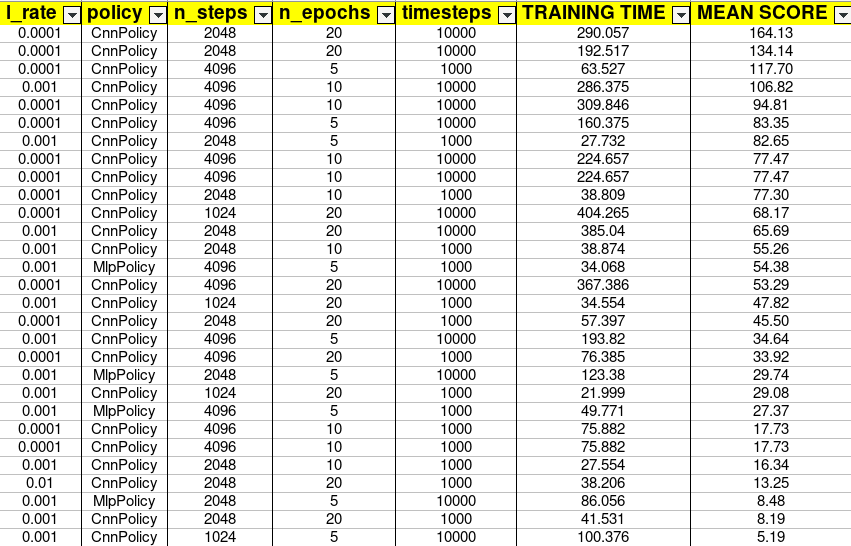
\includegraphics[width=\textwidth]{Screenshots/best30.png}
  \caption{30 Highest mean rewarded networks with their parameters}
  \label{fig:results}
\end{figure}

\begin{figure}
  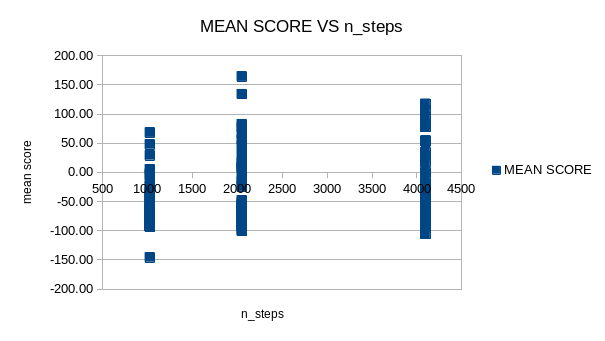
\includegraphics[width=\textwidth]{Screenshots/mean_vs_time.png}
  \caption{The mean award value vs number of steps}
  \label{fig:steps}
\end{figure}

\begin{figure}
  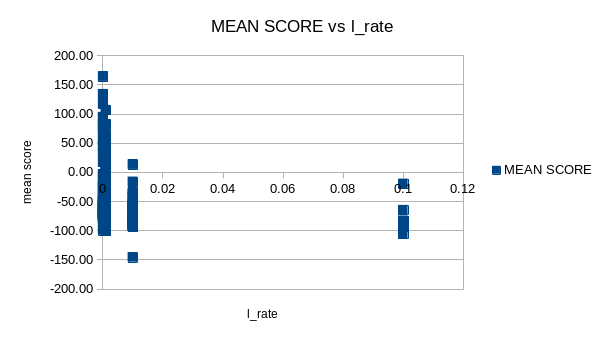
\includegraphics[width=\textwidth]{Screenshots/mean_vs_epochs.png}
  \caption{The mean award value vs learning rate}
  \label{fig:rate}
\end{figure}

\begin{figure}
  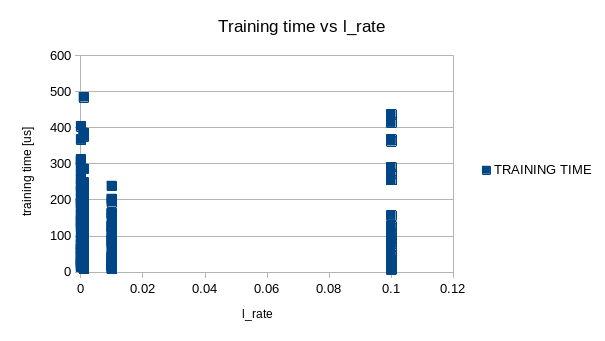
\includegraphics[width=\textwidth]{Screenshots/rate_vs_time.png}
  \caption{learning rate vs time}
  \label{fig:time}
\end{figure}

Finally, the best model was rendered and tested. On the Fig.~\ref{fig:on_track} there can be seen the car being perfectly on track and it's score is increasing, and while it stays on this track it keeps it's position about in the middle of the track. For the further testing the best parameters from the Grid Search algorithm were constant and it was decided to experiment only with the timestep, due to empirical experience. It was observed that the best results were obtained for the timestep increased to $3.5 * 10^5$, which was gained with empirical method. Nevertheless, increase of the timestep not always results in the improved results. For instance with the timestep increased to the $10^6$ the score decreases and in the end game is lost. Finally, the best score was equal to 916, and the game was won successfully as it can be observed in the game won video as well as on the Fig.~\ref{fig:game_won}
\begin{figure}
  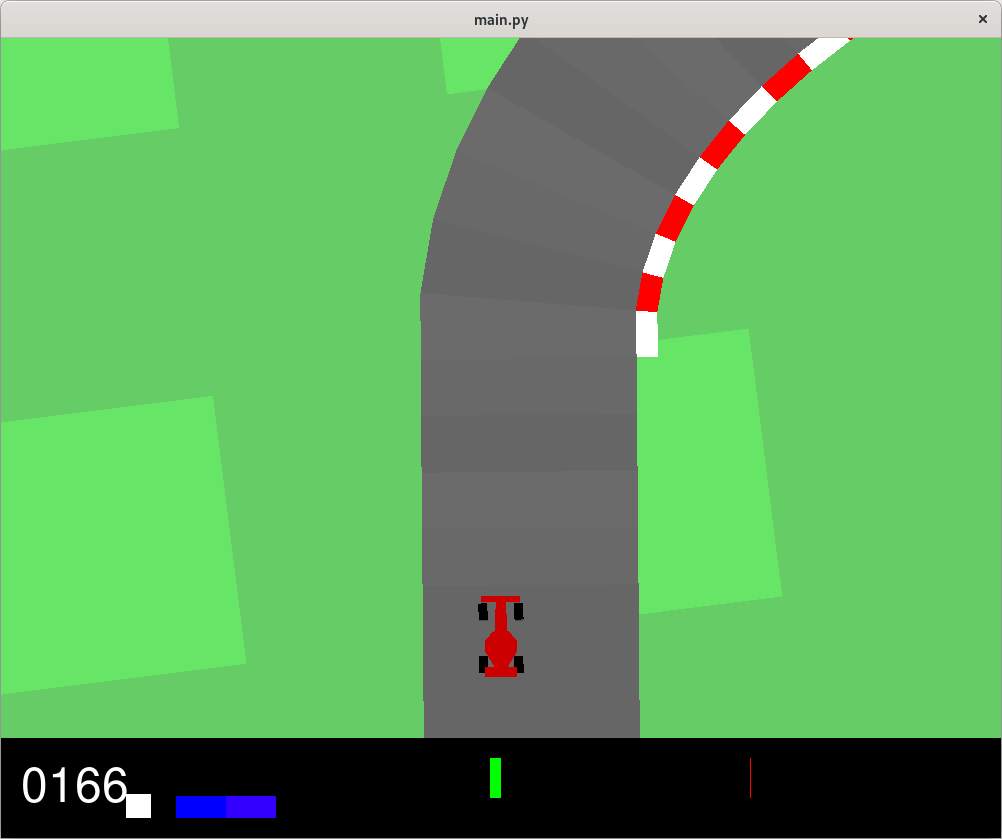
\includegraphics[width=\textwidth]{Screenshots/on_track.png}
  \caption{Initial on track ride}
  \label{fig:on_track}
\end{figure}

\begin{figure}
  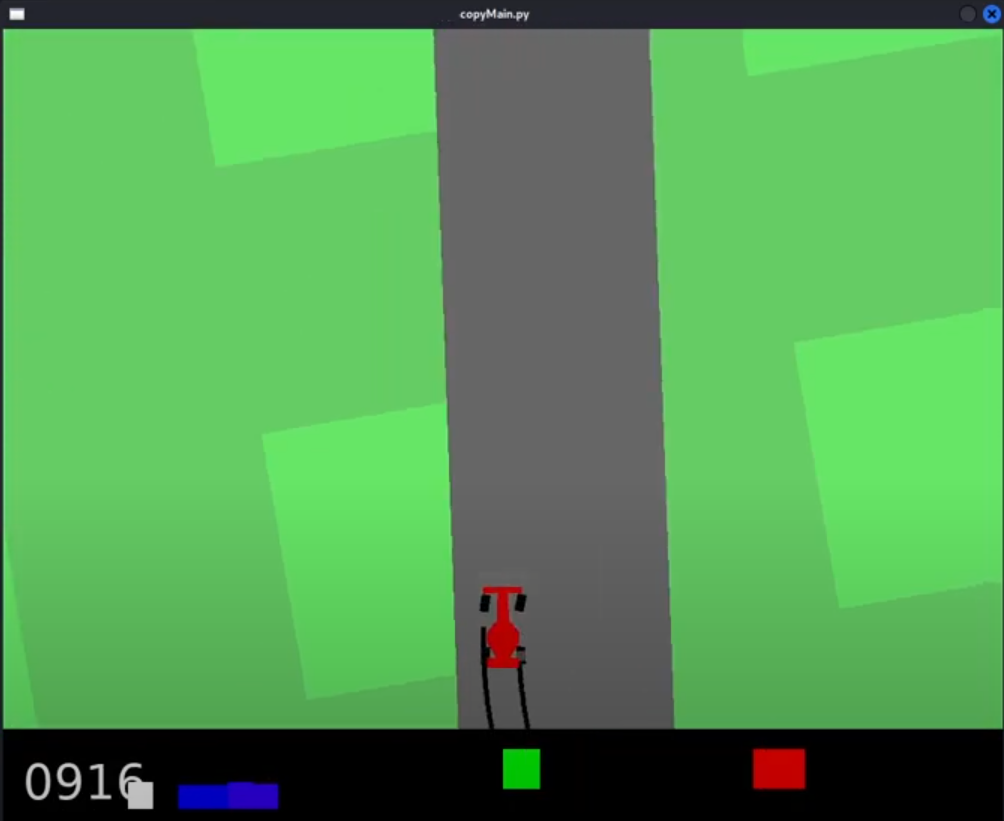
\includegraphics[width=\textwidth]{Screenshots/game_won.png}
  \caption{Game won with the result}
  \label{fig:game_won}
\end{figure}

\end{document}
